
\documentclass[portugues]{DAELT} % Chama a classe DAELT com a opção de idioma em português.

% informações do PDF
\makeatletter
\hypersetup{
	%pagebackref=true,
	pdftitle={\@title}, 
	pdfauthor={Autores},
	pdfsubject={ET76C-Laboratório},
	pdfcreator={LaTeX with abnTeX2},
	pdfkeywords={abnt}{Overleaf}{ET76C}{UTFPR}, 
	colorlinks=true,       		% false: boxed links; true: colored links
	linkcolor=linkcolor,        % color of internal links
	citecolor=citecolor,        % color of links to bibliography
	filecolor=black,      		% color of file links
	urlcolor=linkcolor,
	bookmarksdepth=4
}
\makeatother


%https://creativecommons.org/licenses/by-nc-sa/3.0/br/
\copyrightnotice{CC BY-NC-SA 3.0 BR {\copyright\the\year} UTFPR}
\journalname{\small{ET76C -- LABORATÓRIO DE ELETRÔNICA DE POTÊNCIA}}
\journaldate{\small{\the\year/2}}


\author{Primeiro A. Autor, Segundo B. Autor e Adriano Ruseler\\
	\normalsize Universidade Tecnológica Federal do Paraná -- UTFPR, Curitiba -- PR, Brasil\\	
  \normalsize ORCID: 
  \href{http://orcid.org/0000-0003-0915-9483}{0000-0003-0915-9483} , 
  \href{http://orcid.org/0000-0003-0915-9483}{0000-0003-0915-9483} e 
  \href{http://orcid.org/0000-0003-0915-9483}{0000-0003-0915-9483}\\
  \normalsize e-mail: prime\_iro@alunos.utfpr.edu.br, segundo@alunos.utfpr.edu.br e ruseler@utfpr.edu.br\\
 }

% Título utilizado para nomear o projeto no Overleaf
\title{ET76C-LAB-TurmaA-G00-Exp02} % Coloque aqui a sua turma e grupo;

% Inicia documento 
\begin{document}

% Escolha o arquivo referente ao experimento (Apenas 1)

%
\titulo{INSTRUÇÕES PARA A ELABORAÇÃO DO ARTIGO} % Titulo em português

\title{INSTRUCTIONS FOR PREPARING THE ARTICLE} % Título em inglês

\maketitle

\editorfootnote{Artigo compilado em {\today} às {\currenttime}h, referente ao experimento de número 00 da disciplina de Laboratório de Eletrônica de Potência -- ET76C, ministrada pelo Prof. Adriano Ruseler, Dr. Eng.\\
Colabore: \url{https://www.overleaf.com/10162900nczjmzfrsbdy} }


\begin{resumo}  O resumo deve ser conciso e ao mesmo tempo refletir o que é apresentado no artigo, cujo entendimento deve independer da leitura do trabalho, sem notas de rodapé, abreviações e referências. Deve ser escrito em apenas um parágrafo, de forma impessoal, sem equações ou tabelas. Evite repetir expressões ou utilizar varias vezes a mesma palavra. Busque encadear as frases em um início, meio e fim.
\end{resumo}

\begin{palavraschave }
		Os autores devem apresentar um conjunto de até seis palavras-chave (em ordem alfabética, todas iniciais maiúsculas e separadas por vírgula) que possam identificar os principais tópicos abordados.	
%Use a lista de palavras--chave:\\ \url{http://www.ieee.org/organizations/pubs/ani_prod/keywrd98.txt}	
\end{palavraschave }

\englishtitle

\begin{abstract}
	The abstract must be a concise yet comprehensive reflection of what is in your article, a microcosm of the full article. The abstract must be written as one paragraph, and should not contain displayed mathematical equations or tabular material.  Ensure that your abstract reads well and is grammatically correct.
\end{abstract}

\begin{keywords}
	The abstract should include three or four different keywords or phrases, as this will help readers to find it. It is important to avoid over-repetition of such phrases as this can result in a page being rejected by search engines. For a list of suggested keywords, \url{http://www.ieee.org/organizations/pubs/ani_prod/keywrd98.txt}
\end{keywords}

%\section*{NOMENCLATURA}
%
%\symbolnomenclature{$P$}{Número de polos.}
%\symbolnomenclature{$V_{qd}$}{Componentes $dq$ da tensão de estator.}

\section*{Apresentação geral do trabalho}

\subsubsection{Introdução} 
A introdução deve preparar o leitor para o trabalho propriamente dito, dando uma visão histórica do assunto, e servir como um guia a respeito de como o trabalho está organizado, enfatizando quais são as reais contribuições do mesmo em relação aos já apresentados na literatura. A introdução não deve ser uma repetição do Resumo e deve ser a primeira seção do trabalho a ser numerada como seção.

%\newpage
\subsubsection{Corpo do trabalho} 
Os autores devem organizar o corpo do trabalho em diversas seções, as quais devem conter de forma clara, as informações a respeito do trabalho desenvolvido, facilitando a compreensão do mesmo por parte dos leitores.

\subsubsection{Referências} 
As citações das referências ao longo do texto devem aparecer entre colchetes, antes da pontuação das sentenças nas quais estiverem inseridas. Devem ser utilizados somente os números das referências, evitando-se uso de citações do tipo ``...conforme referência \cite{angulo_active_2013}...''.

Os trabalhos que foram aceitos para publicação, mas que ainda não foram publicados, devem ser colocados nas referências com a citação ``no Prelo''.

Os artigos de periódicos e anais devem ser incluídos iniciando-se pelos nomes dos autores (iniciais seguidas do último sobrenome), seguido do título do trabalho, onde foi publicado (em itálico), número do volume, páginas, mês e ano da publicação. 

No caso de livros, após os autores (iniciais seguidas do último sobrenome), o título deve ser em itálico, seguido da editora, da edição e do local e ano de publicação. 

No final destas normas, é mostrado um exemplo de como devem ser apresentadas as referências \cite{angulo_active_2013,batschauer_three-phase_2012,biela_passive_2009,de_bastiani_lange_three-level_2015,dupczak_space_2012,gong_comparative_2005,heerdt_control_2014,heldwein_novel_2009,heldwein_three-phase_2011,heldwein_implementation_2010,heldwein_impact_2009,heldwein_winding_2008,heldwein_three-phase_2010,heldwein_common_2010,lago_operation_2011,nussbaumer_modeling_2008,nussbaumer_comparison_2008,nussbaumer_differential_2006,ortmann_generalized_2012,rodrigues_three-level_2009,ruiz-caballero_symmetrical_2010,silveira_ortmann_three-phase_2015,silveira_ortmann_high_2014}.


\subsubsection{Dados biográficos} 
Os dados biográficos dos autores deverão estar na mesma ordem de autores colocados no início do trabalho e deverão conter basicamente os seguintes dados:
\begin{enumerate}
	\item Nome Completo (em negrito e sublinhado);
	\item Local e ano de Graduação e Pós-Graduação;
	\item Experiência Profissional (Instituições e empresas em que já trabalhou, número de patentes obtidas, áreas de atuação, atividades científicas relevantes, sociedades científicas a que pertence, etc.). \newline
\end{enumerate}

Caso sejam utilizados os itens adicionais Nomenclatura, Apêndices e Agradecimentos as seguintes instruções devem ser observadas:

\subsubsection{Nomenclatura} 
A nomenclatura consiste na definição das variáveis e símbolos utilizados ao longo do trabalho. Não é obrigatória a sua inclusão e este item não é numerado como seção. Se este item for incluído, deve preceder o item Introdução. Caso os autores optem por não incluir este item, as definições das variáveis e símbolos utilizados devem ser incluídas ao longo do texto, logo após o seu aparecimento. No início destas normas é apresentado um exemplo para este item opcional.

\vspace*{-0.1mm}
\subsubsection{Agradecimentos e apêndices} 
Os agradecimentos a eventuais colaboradores, assim como apêndices, não recebem numeração e devem ser colocados no texto, antes das referências.  No final deste trabalho  é mostrado um exemplo de como podem ser feitos estes agradecimentos.

Na última página do artigo os autores devem distribuir o conteúdo uniformemente, utilizando-se ambas as colunas, de tal forma que estejam paralelas quanto ao fechamento das mesmas.

\subsection{Organização das Seções do Trabalho}

A organização do trabalho em títulos e subtítulos serve para dividi-lo em seções, que ajudam o leitor a encontrar determinados assuntos de interesse dentro do trabalho. Também auxiliam os autores a desenvolverem de forma ordenada seu trabalho. O trabalho deve ser organizado em seções primárias, secundárias e terciárias.

As seções primárias são os títulos de seções propriamente ditos. São grafados em letras maiúsculas no centro da coluna, separadas por uma linha em branco anterior e uma posterior, e utilizam numeração romana e sequencial.

As seções secundárias são os subtítulos das seções. Apenas as primeiras letras das palavras que a compõe são grafadas em letra maiúscula, na margem esquerda da coluna sendo separada do resto do texto por uma linha em branco anterior. A designação das seções secundárias é feita com letras maiúsculas, seguidas de um ponto. Utilizam grafia em itálico.

As seções terciárias são subdivisões das seções secundárias. Apenas a primeira letra da primeira palavra que a compõe é grafada em letra maiúscula. A designação das seções terciárias é feita com algarismos arábicos, seguidos de um parêntese. Utilizam grafia em itálico.



Figuras, tabelas e equações devem obedecer as normas apresentadas a seguir.

\subsection{Figuras e Tabelas}

As tabelas e figuras (desenhos ou reproduções fotográficas) devem ser inseridas no texto logo após serem citadas pela primeira vez, desde que caibam dentro dos limites da coluna; caso necessário, pode-se utilizar toda a área útil da página. A resolução das figuras deve ser superior a 300 dpi e, preferencialmente, no formato vetorial para boa qualidade de impressão. A legenda deve ser situada acima da tabela, enquanto que na figura deve ser colocada abaixo da mesma. As tabelas devem possuir títulos e são designadas pela palavra Tabela, sendo numeradas em algarismos romanos, sequencialmente. As legendas das tabelas devem estar centralizadas e em negrito.  

%\newpage
As figuras necessitam de legenda, e são designadas pela palavra Figura no texto (Fig. na própria legenda), numeradas em algarismos arábicos, sequencialmente, com alinhamento justificado conforme exemplo. A designação das partes de uma figura é feita pelo acréscimo de letras minúsculas ao número da figura, começando pela letra a, como por exemplo, \figref{fig:fig1}.

\begin{figure}[!t]
	\centering
    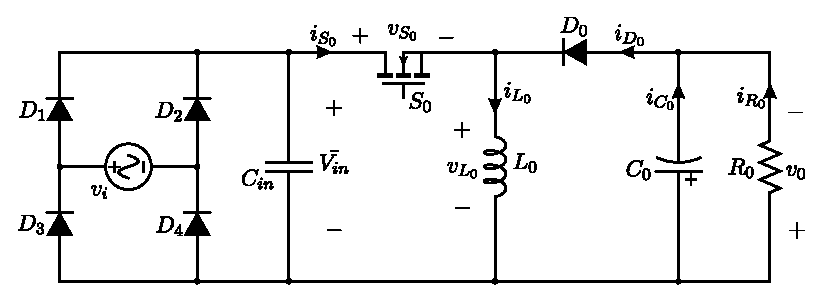
\includegraphics[width=0.9\linewidth]{Figs/RET-BuckBoost}
	\caption{Conversor Buck-Boost. (Observe que o termo ``Fig.'' é abreviado. Existe um ponto após o número da figura, seguido de dois espaços antes da legenda).}
	\label{fig:BuckBoost}
\end{figure}



Com o intuito de facilitar a compreensão dos gráficos, a definição dos eixos dos mesmos deve ser feita utilizando-se palavras e não letras, exceto no caso de formas de onda e planos de fase. As unidades devem ser expressas entre parênteses.~Por exemplo, utilize a denominação ``Magnetização (A/m)'', ao invés de ``M (A/m)''.

As figuras e tabelas devem ser posicionadas preferencialmente no início ou no final das colunas, evitando-as no meio das colunas. Devem ser evitadas tabelas e figuras, cujas dimensões ultrapassem as dimensões das colunas. As figuras devem ser preferencialmente editadas em preto, em fundo branco, uma vez que a versão impressa da revista não utiliza cores. Os traços devem ser de espessura tal que permitam uma impressão legível.



\begin{table}[!ht]
	\centering
	\caption{\textbf{Tamanhos e Tipos de Letras Utilizadas no Texto}}
	\footnotesize
	\setlength{\tabcolsep}{5pt}
	\begin{tabular}{cccc}
		\toprule [1.3pt]	
		\multicolumn{4}{c}{ \textbf{Estilo} } \\
		\hline
		\multirow{2}{1.1cm}{\centering \textbf{Tamanho (pontos)}} & \multirow{2}{*}{\textbf{Normal}} &
		\multirow{2}{*}{\textbf{Negrito}} & \multirow{2}{*}{\textbf{Itálico}} \\
		&  &  & \\		
		\hline
		8 & Texto de tabelas &  &  \\
		\hline
		\multirow{2}{*}{9} & \multirow{2}{2cm}{\centering Legendas de figuras}  &  &  \\
		& & & \\
		\hline
		\multirow{3}{*}{10} &  
		\multirow{3}{2cm}{\centering Instituição dos autores; texto em geral; referências}  & 
		\multirow{3}{2cm}{\centering Textos do resumo e palavras-chave; títulos de tabelas} & 
		\multirow{3}{2.1cm}{\centering Títulos do resumo e palavras-chave} \\
		& &  &  \\
		& &  &  \\
		\hline
		\multirow{2}{*}{12} & \multirow{2}{2cm}{\centering Nomes dos autores}  & \multirow{2}{*}{Título em inglês} &  \\
		& & & \\
		\hline
		14 &  & Título do trabalho & \vspace*{-0.8mm}\\
		\bottomrule[1.3pt]
	\end{tabular} \label{table:TabelaI}
\end{table}


\subsection{Abreviações e Siglas}

As abreviações a serem utilizadas no texto, devem ser definidas na primeira vez em que aparecerem, como por exemplo, ``... Modulação por Largura de Pulso  (PWM)... ''.

\subsection{Equações}

A numeração das equações deve ser colocada entre parênteses, na margem direita, como em \eqnref{eq:eq01}. As equações devem ser editadas de forma compacta e estar centralizadas na coluna. Caso a seção de nomenclatura não seja usada no início do texto, as variáveis devem ser definidas logo após as equações em que são indicadas, tal como:

\begin{equation}\label{eq:eq01}
\Delta I_{L}=I_{o}+\frac{\sqrt{3}}{2}\frac{V_{i}}{Z}
\end{equation} 
onde: 

\symboldescription{$\Delta I_{L}$}{corrente de pico no indutor ressonante;}
\symboldescription{$I_o$}{corrente de carga;}
\symboldescription{$V_i$}{tensão de alimentação;}
\symboldescription{$Z$}{impedância característica do circuito ressonante.}


\subsection{Discussões}
A seção de Discussão, muitas vezes a mais difícil de escrever, deverá ser relativamente fácil se as sugestões anteriores forem seguidas. Em particular, olhar para o último parágrafo da introdução. Se o trabalho caracterizou um fenômeno ao estudar os efeitos específicos, usar os resultados para descrever cada efeito em parágrafos separados. Se o trabalho apresentou uma hipótese, usar os resultados para construir um argumento lógico que apoia ou rejeita sua hipótese. Se o trabalho identificou três objetivos principais para o trabalho, usar os resultados para abordar cada um desses objetivos. Um estudo bem definido, que é descrito na Introdução, juntamente com o apoio de resultados que são apresentados na seção de Resultados, deverá aliviar a construção da seção de Discussão.

Comece a seção de Discussão com um breve parágrafo que novamente dará uma visão geral para o trabalho. Resumir os resultados mais importantes e, se for o caso, aceitar ou rejeitar a hipótese proposta. Em seguida, identificar os mais interessantes, significativos resultados notáveis que foram apresentados
na seção de Resultados e contrastar estes resultados à luz de outros estudos relatados na literatura. É frequentemente informativo se uma discussão sobre os possíveis pontos fracos da interpretação também estiver incluída. Finalmente, no final da seção de Discussão, considere os outros trabalhos na literatura que abordam este tema e como este trabalho contribui para o campo geral do estudo.

\bibliographystyle{IEEEtran}

\bibliography{Refs/References} % Inclui arquivos de referência

\balance



\titulo{RETIFICADOR DE ONDA COMPLETA COM FILTRO CAPACITIVO} % Titulo em português

\title{FULL WAVE RECTIFIER WITH CAPACITIVE FILTER} % Título em inglês

\maketitle

\editorfootnote{Artigo compilado em {\today} às {\currenttime}h, referente ao experimento de número 01 da disciplina de Laboratório de Eletrônica de Potência -- ET76C, ministrada pelo Prof. Adriano Ruseler, Dr. Eng.\\
Colabore: \url{https://www.overleaf.com/10162900nczjmzfrsbdy} }



\begin{resumo}  O resumo deve ser conciso e ao mesmo tempo refletir o que é apresentado no artigo, cujo entendimento deve independer da leitura do trabalho, sem notas de rodapé, abreviações e referências. Deve ser escrito em apenas um parágrafo, de forma impessoal, sem equações ou tabelas. Evite repetir expressões ou utilizar varias vezes a mesma palavra. Busque encadear as frases em um início, meio e fim.
\end{resumo}

\begin{palavraschave }
		Os autores devem apresentar um conjunto de até seis palavras-chave (em ordem alfabética, todas iniciais maiúsculas e separadas por vírgula) que possam identificar os principais tópicos abordados.	
%Use a lista de palavras--chave:\\ \url{http://www.ieee.org/organizations/pubs/ani_prod/keywrd98.txt}	
\end{palavraschave }

\englishtitle

\begin{abstract}
	The abstract must be a concise yet comprehensive reflection of what is in your article, a microcosm of the full article. The abstract must be written as one paragraph, and should not contain displayed mathematical equations or tabular material.  Ensure that your abstract reads well and is grammatically correct.
\end{abstract}

\begin{keywords}
	The abstract should include three or four different keywords or phrases, as this will help readers to find it. It is important to avoid over-repetition of such phrases as this can result in a page being rejected by search engines. For a list of suggested keywords, \url{http://www.ieee.org/organizations/pubs/ani_prod/keywrd98.txt}
\end{keywords}




%\section*{NOMENCLATURA}
%
%\symbolnomenclature{$P$}{Número de polos.}
%\symbolnomenclature{$V_{qd}$}{Componentes $dq$ da tensão de estator.}


% Introdução
\section{INTRODUÇÃO}


A seção de Introdução tem o objetivo geral de apresentar a natureza do problema abordado no trabalho, através de adequada revisão bibliográfica, o propósito e a contribuição do artigo submetido.

A introdução requer uma breve revisão da literatura referente ao tópico de pesquisa. A introdução é então melhor construída como um funil descritivo, começando com temas gerais e focando lentamente no trabalho em questão. Talvez de três a quatro parágrafos sejam necessários. Uma abordagem pode ser começar com um ou dois parágrafos que introduzam o leitor para o estudo de campo geral. Os parágrafos subsequentes então descrevem como um aspecto deste campo poderia ser melhorado. O parágrafo final é essencial. Ele afirma claramente, provavelmente na primeira frase do parágrafo, qual questão experimental será respondida pelo estudo. A hipótese é então indicada. Em seguida, descreve brevemente a abordagem que foi feita para testar a hipótese. Finalmente, uma frase de resumo pode ser adicionada informando como a resposta da sua pergunta vai contribuir para o campo geral de estudo.

\begin{enumerate}
\item Contextualização do assunto/problema apresentado no artigo
	\begin{enumerate}
		\item Explicar o que é um retificador, conceitos básicos, CC, CA...
		%		\item Explique os conceitos básicos, CC, CA...		
	\end{enumerate}									
\item Breve revisão da literatura referente ao tópico do experimento
	\begin{enumerate}
		\item Buscar topologias utilizadas como retificadores. Cite alguma referência.
		%		\item Explique os conceitos básicos, CC, CA...		
	\end{enumerate}	
\item Apresentação da abordagem adotada e solução sugerida
	\begin{enumerate}
		\item Apresente a estrutura estudada e montada (ver \figref{fig:retondacompletarc}).
	\end{enumerate}	
	\end{enumerate}	


\begin{figure}[!hb]
	\centering
	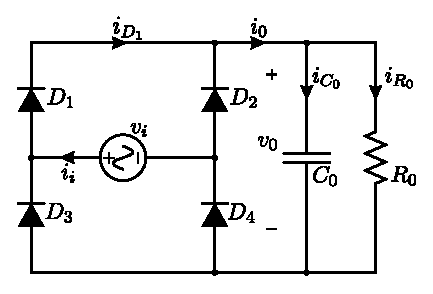
\includegraphics[width=0.65\linewidth]{Figs/RetOndaCompletaRC}
	\caption{Retificador de onda completa com filtro capacitivo.}
	\label{fig:retondacompletarc}
\end{figure}






\section{Estudo teórico}

Esta seção tem o objetivo de apresentar o embasamento teórico necessário para o entendimento da solução apresentada (ver Planilha).
\begin{enumerate}									
	\item  Apresente a expressão para o cálculo da ondulação da tensão de saída ($\Delta V_{C0}$).
	\item Apresente a expressão para o cálculo do valor médio da tensão de saída ($\bar{V_0}$).
	\item  Apresente a expressão para o cálculo do ângulo de condução do diodo $D_1$ ($\gamma_D$) e do tempo de condução do mesmo ($t_D$).
	\item  Apresente a expressão para o cálculo do valor de pico da corrente de carga ($\hat{I_0}$), valor médio ($\bar{I_0}$).
	\item Apresente a expressão para o fator de crista, ou seja, a relação do valor de pico da corrente de carga ($\hat{I_0}$) pelo valor eficaz (${I_0}$).
	
	\item Apresente a expressão para o cálculo do fator de potência da estrutura.
	
\end{enumerate}


\section{Verificação por simulação}


A análise teórica apresentada anteriormente deve ser verificada por simulação.
\begin{enumerate}									
	\item   Apresente as formas de onda da tensão de saída em comparação com a tensão de saída sem o capacitor de filtro $|\sin(\omega_0 t)|$. Verifique o valor médio obtido por simulação com o teórico.
	\item   Apresente as formas de onda da corrente ($i_i$) de entrada e no diodo $D_1$. Verifique o cálculo do valor de pico e do valor médio.
	\item   Verifique o cálculo do tempo de condução do diodo.
	\item   Verifique o cálculo do fator de potência da estrutura.
	\item  Comente sobre as aproximações realizadas, dependendo dos parâmetros, por exemplo, sem a resistência de entrada (\emph{shunt}) a corrente de carga tem um formato triangular. Com a adição da resistência de entrada, a corrente passa a ter um formato senoidal.
\end{enumerate}





%Body Text
\section{Resultados experimentais}


A análise teórica, assim como as simulações, são verificadas de forma definitiva com os resultados experimentais.
\begin{enumerate}									
	\item   Descrever o experimento. Listar o material utilizado.  
	\item  Verificar experimentalmente cada item simulado na seção anterior;
	\item  Apresente uma fotografia do protótipo montado;
	\item  Salve as aquisições em formato .png e as coloque aqui, afim de verificar a operação adequada do retificador.
\end{enumerate}

A \tabref{tab:componentes} apresenta a lista de componentes utilizados...

\begin{table}[!hb]
	\centering
	\caption{Componentes utilizados}
	\label{tab:componentes}
	\begin{tabular}{@{}ccc@{}}
		\toprule
		\textbf{Componente} & \textbf{Descrição} & \textbf{Quantidade} \\ \midrule
		Resistores          & \SI{820}{\ohm} -- \SI{5}{\W}             & 4                   \\
		Resistor shunt      & \SI{0.1}{\ohm} -- \SI{5}{\W}             & 2                   \\
		Diodos              & 1N4007             & 4                   \\
		Capacitor           & \SI{220}{\micro\farad} x \SI{250}{\V}      & 1                   \\
		Conector Borne      &  KRE 2 Vias    & 2                   \\
		Fusível/Porta Fusível     &  \SI{5}{\A}  & 1                  \\
		Placa padrão        & \SI{10}{\cm} por \SI{10}{\cm}         & 1                   \\ \bottomrule
	\end{tabular}
\end{table}



\section{Conclusões} 

Por fim, apresenta-se uma conclusão sobre o trabalho estudado.
\begin{enumerate}								
	\item  Desfecho do trabalho. Problemas encontrados, soluções alcançadas...
	\item  Análise crítica, sugestões...
	%	\bonuspart[01] Parte extra.		
\end{enumerate}


As conclusões devem ser as mais claras possíveis, informando aos leitores sobre a importância do trabalho dentro do contexto em que se situa. As vantagens e desvantagens em relação aos já existentes na literatura devem ser comentadas, assim como os resultados obtidos e as possíveis aplicações práticas do trabalho.


\bibliographystyle{IEEEtran}

\bibliography{References} % Inclui arquivos de referência

\balance



%\titulo{MODULADOR POR LARGURA DE PULSO} % Titulo em português

\title{PULSE WIDTH MODULATOR} % Título em inglês

\maketitle

\editorfootnote{Artigo compilado em {\today} às {\currenttime}h, referente ao experimento de número 02 da disciplina de Laboratório de Eletrônica de Potência -- ET76C, ministrada pelo Prof. Dr. Adriano Ruseler, Eng.\\
Repositório: \url{https://github.com/AdrianoRuseler/ET76C-LAB} }



\begin{resumo}  O resumo deve ser conciso e ao mesmo tempo refletir o que é apresentado no artigo, cujo entendimento deve independer da leitura do trabalho, sem notas de rodapé, abreviações e referências. Deve ser escrito em apenas um parágrafo, de forma impessoal, sem equações ou tabelas. Evite repetir expressões ou utilizar varias vezes a mesma palavra. Busque encadear as frases em um início, meio e fim.
\end{resumo}

\begin{palavraschave }
		Os autores devem apresentar um conjunto de até seis palavras-chave (em ordem alfabética, todas iniciais maiúsculas e separadas por vírgula) que possam identificar os principais tópicos abordados.	
%Use a lista de palavras--chave:\\ \url{http://www.ieee.org/organizations/pubs/ani_prod/keywrd98.txt}	
\end{palavraschave }

\englishtitle

\begin{abstract}
	The abstract must be a concise yet comprehensive reflection of what is in your article, a microcosm of the full article. The abstract must be written as one paragraph, and should not contain displayed mathematical equations or tabular material.  Ensure that your abstract reads well and is grammatically correct.
\end{abstract}

\begin{keywords}
	The abstract should include three or four different keywords or phrases, as this will help readers to find it. It is important to avoid over-repetition of such phrases as this can result in a page being rejected by search engines. For a list of suggested keywords, \url{http://www.ieee.org/organizations/pubs/ani_prod/keywrd98.txt}
\end{keywords}

%\section*{NOMENCLATURA}
%
%\symbolnomenclature{$P$}{Número de polos.}
%\symbolnomenclature{$V_{qd}$}{Componentes $dq$ da tensão de estator.}


% Introdução
\section{INTRODUÇÃO}


A seção de Introdução tem o objetivo geral de apresentar a natureza do problema abordado no trabalho, através de adequada revisão bibliográfica, o propósito e a contribuição do artigo submetido.

A introdução requer uma breve revisão da literatura referente ao tópico de pesquisa. A introdução é então melhor construída como um funil descritivo, começando com temas gerais e focando lentamente no trabalho em questão. Talvez de três a quatro parágrafos sejam necessários. Uma abordagem pode ser começar com um ou dois parágrafos que introduzam o leitor para o estudo de campo geral. Os parágrafos subsequentes então descrevem como um aspecto deste campo poderia ser melhorado. O parágrafo final é essencial. Ele afirma claramente, provavelmente na primeira frase do parágrafo, qual questão experimental será respondida pelo estudo. A hipótese é então indicada. Em seguida, descreve brevemente a abordagem que foi feita para testar a hipótese. Finalmente, uma frase de resumo pode ser adicionada informando como a resposta da sua pergunta vai contribuir para o campo geral de estudo.

\begin{enumerate}
\item Contextualização do assunto/problema apresentado no artigo
	\begin{enumerate}
		\item Explicar o que é PWM, para o que serve.
		\item Ilustrar a geração com portadora dente de serra.
		\item  Explique os conceitos básicos, razão cíclica, tempo morto...		
	\end{enumerate}									
\item Breve revisão da literatura referente ao tópico do experimento
	\begin{enumerate}
		\item Apresentar formas de se implementar um modulador PWM.
		\item Procurar convergir para o caso estudado UC3525.	
	\end{enumerate}	
\item Apresentação da abordagem adotada e solução sugerida
	\begin{enumerate}
		\item Explique de forma breve o que será apresentado.
		\item Apresente o esquemático implementado.
		\item  Desfecho da introdução e ligação com a seção seguinte (Estudo teórico).
	\end{enumerate}	
	\end{enumerate}	





\section{Estudo teórico}

Esta seção tem o objetivo de apresentar o embasamento teórico necessário para o entendimento da solução apresentada (ver Planilha). 
\begin{enumerate}	
	\item Cálculo para a escolha do resistor $R_T$, com capacitor $C_T$ previamente escolhido para uma determinada frequência de comutação. 								
	\item  Cálculo do capacitor de \textit{soft-start}.	
	\item Cálculo do resistor de gate, supondo o uso do MOSFET IRF740.	
	\item  Dimensionamento e verificação dos limites de razão cíclica.	
\end{enumerate}


\section{Verificação por simulação}


A análise teórica apresentada anteriormente deve ser verificada por simulação. 
 
\begin{enumerate}									
	\item   Apresente as formas de onda responsáveis pela geração do pulso PWM.
	\begin{enumerate}
		\item Sinal portador (Tensão sobre o capacitor $C_T$);
		\item Sinal de comparação (Tensão no ponto médio do Trimpot);
		\item PWM gerado (Tensão sobre o diodo Zener).
	\end{enumerate}
	\item  Verifique o equacionamento para uma razão cíclica em torno de $0,5$.
\end{enumerate}





%Body Text
\section{Resultados experimentais}


A análise teórica, assim como as simulações, são verificadas de forma definitiva com os resultados experimentais.
\begin{enumerate}									
	\item   Descrever o experimento. Listar o material utilizado.  
	\item  Verificar experimentalmente cada item simulado na seção anterior;
	\item  Apresente uma fotografia do protótipo montado;
	\item  Salve as aquisições em formato .png e as coloque aqui, afim de verificar a operação adequada do modulador PWM.
\end{enumerate}

A \tabref{tab:componentesPWM} apresenta a lista de componentes utilizados...

\begin{table}[!ht]
	\centering
	\caption{Componentes utilizados na montagem do modulador PWM}
	\label{tab:componentesPWM}
	\begin{tabular}{@{}ccc@{}}
		\toprule
		\textbf{Componente} & \textbf{Descrição} & \textbf{Quantidade} \\ \midrule			
		Capacitor eletrolítico          & \SI{10}{\micro\farad} x \SI{25}{\V}      & 2  \\		
		Capacitor eletrolítico          & \SI{100}{\micro\farad} x \SI{35}{\V}      & 1  \\
		Capacitor cerâmico          & \SI{10}{\nano\farad} x \SI{25}{\V}      & 2  \\
			CI - PWM      & UC3525 ou SG3525            & 1                   \\
			Conector       & KRE   & 1    \\
				Diodo              & 1N4148             & 2                   \\
			Diodo   Zener          &  \SI{18}{\V} -- \SI{1}{\W}              & 1        \\
				Placa padrão (Reuso)        & \SI{10}{\cm} por \SI{10}{\cm}         & 1    \\
				Resistor  $R_D$     & \SI{10}{\ohm} -- \SI{1/4}{\W}    & 1    \\	
		 Resistor   $R_g$    & \SI{22}{\ohm} -- \SI{1/4}{\W}    & 1    \\
	    Resistor  $R_{pd}$     & \SI{1}{\kilo\ohm} -- \SI{1/4}{\W}    & 2     \\	     
	       Resistor  $R_T$     & \SI{6.8}{\kilo\ohm} -- \SI{1/4}{\W}    & 1    \\
	        Resistor  $R_1$     & \SI{10}{\kilo\ohm} -- \SI{1/4}{\W}    & 1    \\ 
	       Resistor  $R_3$     & \SI{5.6}{\kilo\ohm} -- \SI{1/4}{\W}    & 1    \\              
	          	Soquete para CI        & 16 pinos           & 1                   \\
	       	Transistor    NPN          & BC 548             & 1          \\
	       Transistor    PNP          & BC 558             & 1          \\
	          Trimpot       & \SI{10}{\kilo\ohm}    & 1    \\  \bottomrule	
	\end{tabular}
\end{table}



\section{Conclusões} 

Por fim, apresenta-se uma conclusão sobre o trabalho estudado.
\begin{enumerate}								
	\item  Desfecho do trabalho. Problemas encontrados, soluções alcançadas...
	\item  Análise crítica, sugestões...	
\end{enumerate}


As conclusões devem ser as mais claras possíveis, informando aos leitores sobre a importância do trabalho dentro do contexto em que se situa. As vantagens e desvantagens em relação aos já existentes na literatura devem ser comentadas, assim como os resultados obtidos e as possíveis aplicações práticas do trabalho.


\bibliographystyle{IEEEtran}

\bibliography{References} % Inclui arquivos de referência

\balance




\end{document}


